In this chapter, the product architecture is described using the 4 + 1 architectural view model \cite{Kruchten:1995:VMA:624610.625529}. It is based on the multiple concurrent views and therefore better explanation of architecture can be provided.
Only the high level design will be presented in this chapter and in each sprint. The specific and detailed architecture will be described.
The design is made with emphasis on generality, therefore it is possible, that in particular sprints in the architecture section it will be adapted to specific situation.

Since some design patterns were used, the purpose of using this specific pattern and its advantages will be discussed in the end of this chapter.

\section{Logical view}
The logical view  primarily describes functional requirements \cite[p.~3]{Kruchten:1995:VMA:624610.625529}. 
The client and the server are decomposed into a set of key abstractions, taken from the problem domain, in the form of classes. 

The logical view will be described by class diagrams.
Only core classes will be discussed. 
Detailed architecture of particular parts will be presented in sprint chapters.

You can see server class diagram in Figure \ref{fig:architecture_class_diagram_server}.
As a starting point in this diagram can be considered instance of class \texttt{MainActivityServer}.
This class is controller of whole application and handles inputs by manager.
It also initialize one of the core classes -- \emph{ConnectionService}.
Instance of this class has ability to send commands to clients using methods such as \texttt{broadcast} or \texttt{unicast}, and it is responsible for creating a service on local network.
Its interface is used through whole system.
\begin{figure}[!h]
	\centering
		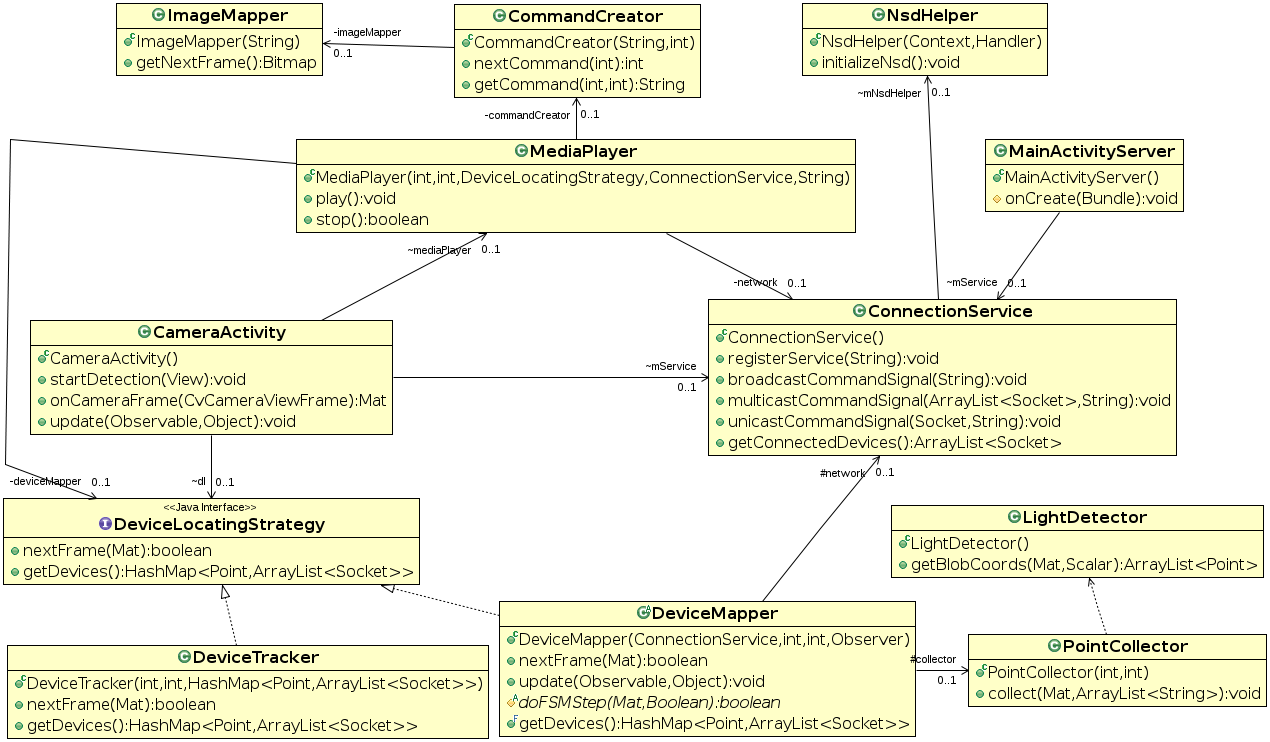
\includegraphics[width=20cm, angle=90]{softwareArchitecture/class_diagram_server.png}
	\caption{Server class diagram}
	\label{fig:architecture_class_diagram_server}
\end{figure}

When inputs from the camera is needed, the instance of class \texttt{CameraActivity} is emerged.
Since that moment, it takes responsibility for all handling inputs from manager and also for displaying feedback of other components on the application screen.
Mentioned class serves only as intermediary between camera and instance of class which implements interface \texttt{DeviceLocatingStrategy}.
This object can process incoming images and according to them it updates its inner data structure, which maps sockets into position on grid.
Two classes implements that interface: \texttt{DeviceMapper} and \texttt{DeviceTracker}.
First mentioned one is used initially, when there are no assumptions about devices positions.
After \texttt{DeviceMapper} assigns position to each socket, his role is taken by \texttt{DeviceTracker}, which is designed\footnote{This class is actually not implemented due to time restriction after discussion with customer. It is only prepared for future extension.} to be able to track movement of devices in time and track the changing position.

Instance of class \texttt{MediaPlayer} provides interface to load a media from a given path and start and stop playing that media.

You can see client class diagram in Figure \ref{fig:architecture_class_diagram_client}.
Instance of class \texttt{MainActivity} handles inputs from user and controls the flow of the whole application.
\texttt{SNTPClient} is a class that main responsibility is to synchronize time through network with other devices.
Instance of class \texttt{Connection} is responsible for connecting to an existing server and also for handling incoming control commands.
These commands are interpreted by instance of class \texttt{ClientPlayer}.

\begin{figure}[!h]
	\centering
		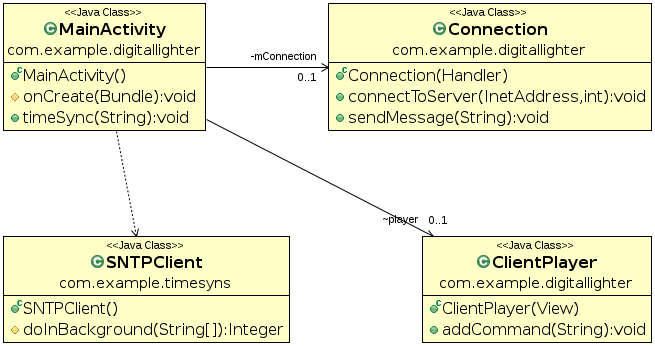
\includegraphics[width=10cm]{softwareArchitecture/class_diagram_client.png}
	\caption{Client class diagram}
	\label{fig:architecture_class_diagram_client}
\end{figure}


\section{Development view}
The development view, is a view of  the system's architecture.It can be described by a component diagram.
It focuses on software module organization in development.
Component diagram shows components in system and their provided and required interfaces.

Component diagram for server application can be seen in Figure \ref{fig:component_diagram_server}.
There are five components: \emph{Network}, \emph{Media player},  \emph{Device locating}, \emph{Device detection}, and \emph{Core}.

\begin{figure}[h]
	\centering
		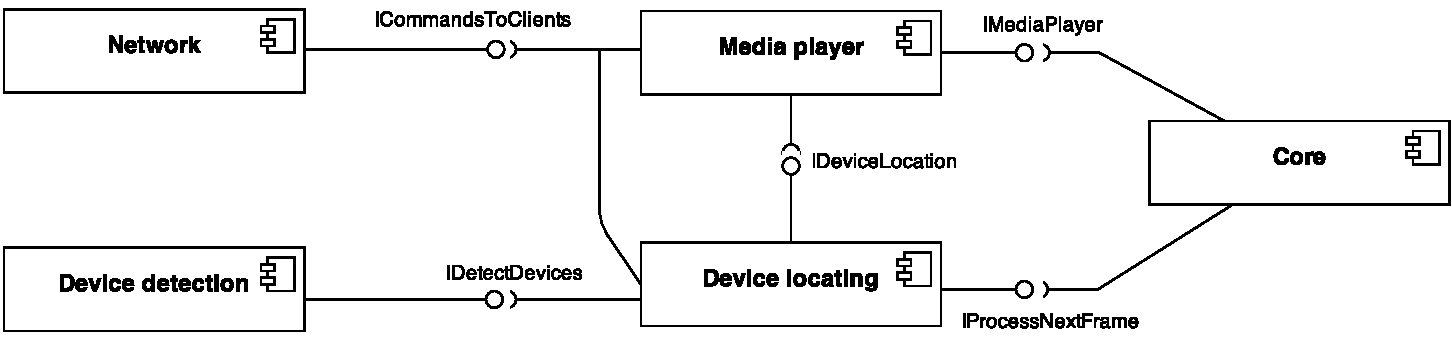
\includegraphics[width=16.2cm]{softwareArchitecture/component_diagram.pdf}
	\caption{Component diagram of server application}
	\label{fig:component_diagram_server}
\end{figure}

\paragraph{Network} is a component that provides interface which allows other components to communicate with clients. 
This includes broadcasting, unicasting and multicasting. 
It is also responsible for handling the new connections from clients and creating new service.

\paragraph{Media player} is a component that provides simple interface consisting of start and stop command. 
It is responsible for playing actual media and timing for sending control commands to clients.

\paragraph{Device locating} is a component providing two interfaces. 
It must be able to handle incoming images and also it provides to other components locations of all connected clients.

\paragraph{Device detection} is a component that provides single interface. 
It accepts image as an input and it returns positions of possible devices.

\paragraph{Core} is a component that handles camera and manager's actions.

Component diagram for client application can be seen in Figure \ref{fig:component_diagram_client}.
There are four components: \emph{Network}, \emph{Command player},  \emph{Time synchronization}, and \emph{Core}.
\begin{figure}[h]
	\centering
		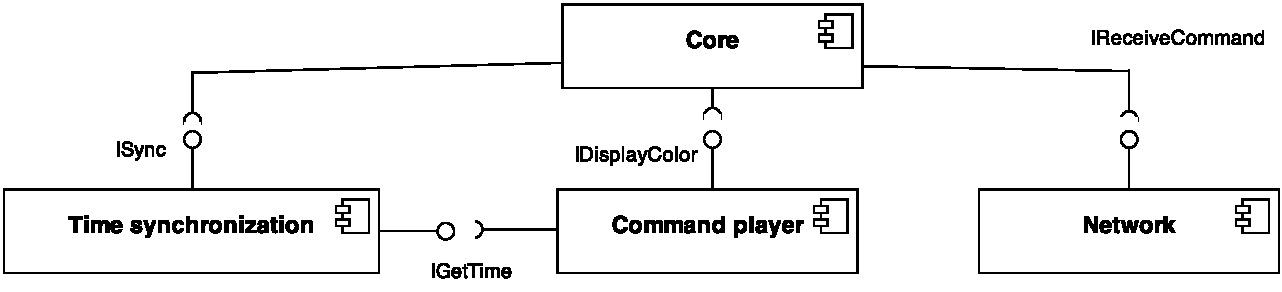
\includegraphics[width=13cm]{softwareArchitecture/component_diagram_client.pdf}
	\caption{Component diagram of client application}
	\label{fig:component_diagram_client}
\end{figure}

\paragraph{Network} is a component that provides interface for receiving control commands.
It is also responsible for connecting to server.

\paragraph{Command player} is a component that provides interface for displaying color at certain time in screen.
Therefore it also requires access to synchronized current time.

\paragraph{Time synchronization} as a component that provides two interfaces. 
\emph{ISync} is an interface through time synchronization with remote server can be started.
\emph{IGetTime} interface provides current synchronized time.

\paragraph{Core} is a component which handles client user's actions and requires several interfaces, mention above.

\section{Process view}
The process view shows concurrency and distribution of a system and system's processes.
It can also show communication between these units.
Process view can be described by activity diagrams.

You can see activity diagrams in Figures \ref{fig:activity_diagram_server} and \ref{fig:activity_diagram_client}. Note, that client application is sending signal action \emph{connect to server}, which is connected to server's event action \emph{new client connected}. 
 All clients connections are stored in data store \emph{client list} and particular actions require all client connections to be able to send any information to clients.

\begin{figure}[h]
	\centering
		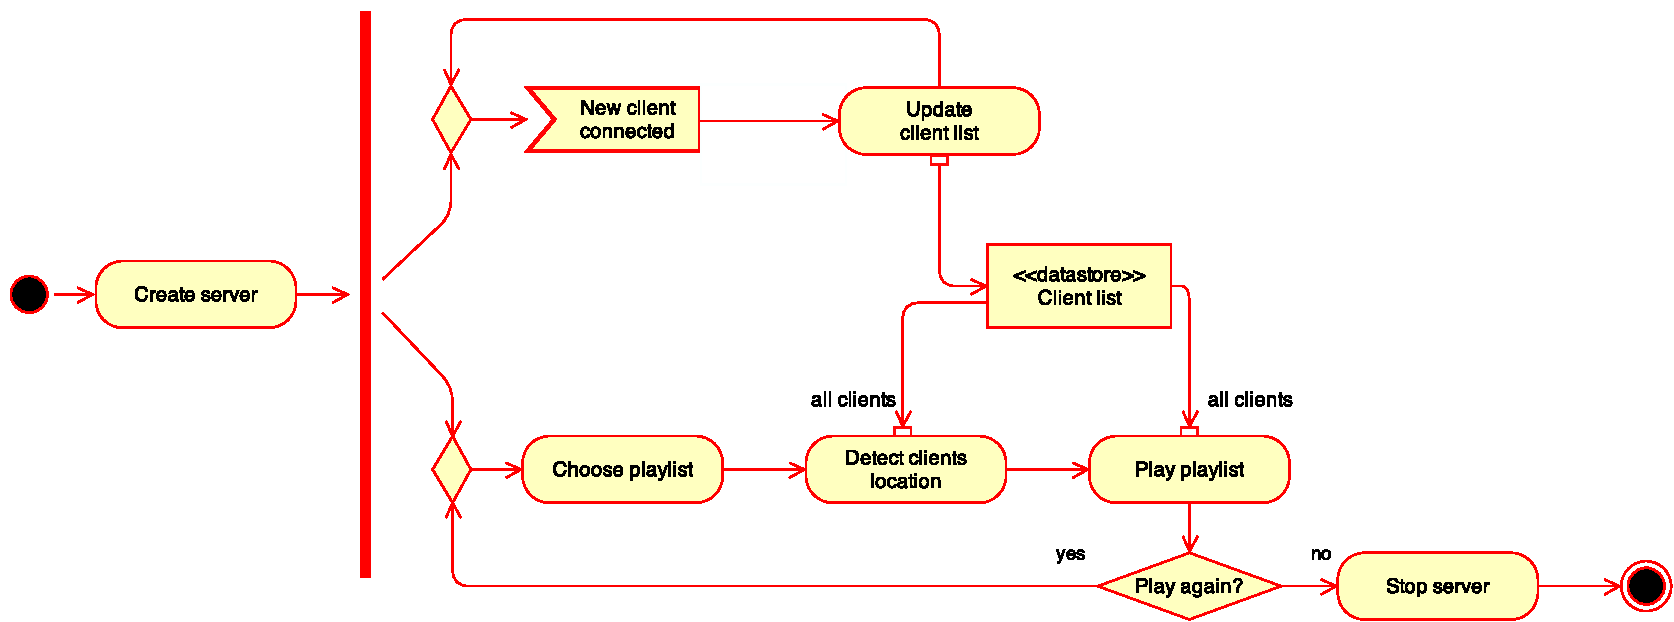
\includegraphics[width=16.2cm]{softwareArchitecture/activity_server.pdf}
	\caption{Activity diagram of server application}
	\label{fig:activity_diagram_server}
\end{figure}

\begin{figure}[h]
	\centering
		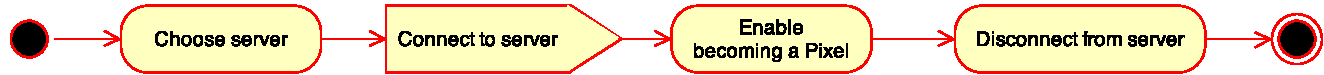
\includegraphics[width=16.2cm]{softwareArchitecture/activity_client.pdf}
	\caption{Activity diagram of client application}
	\label{fig:activity_diagram_client}
\end{figure}


\section{Physical view}
The physical view \cite{Kruchten:1995:VMA:624610.625529} describes a mapping of software onto hardware. 
It takes into account the non-functional requirements of the system, and it can be described by deployment diagrams.

Deployment diagram depicting physical view can be seen in Figure \ref{fig:architecture_deployment_diagram}.
According to requirement \refreq{N1}, there are two executable files deployed; one deployed to client device and second to server device.
There is also need for NTP\footnote{\url{http://ntp.org/}} server, which will maintain all connected devices synchronized.
To generalize the architecture design, the \emph{camera} device is treated as a separate device, which will only send its output to server device.

\begin{figure}[h]
	\centering
		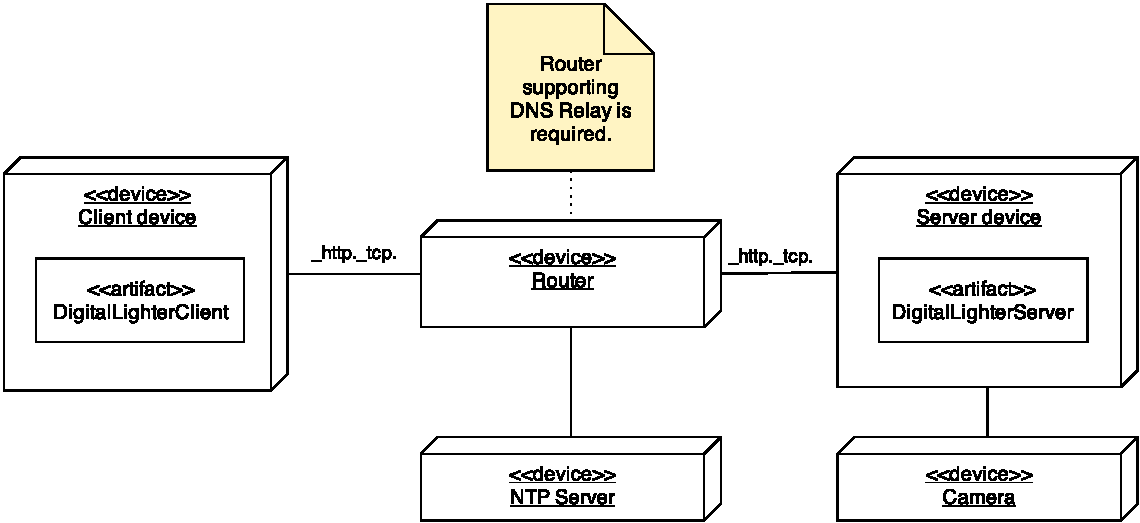
\includegraphics[width=15cm]{softwareArchitecture/deployment-diagram.pdf}
	\caption{Deployment diagram}
	\label{fig:architecture_deployment_diagram}
\end{figure}

\section{Scenarios}
Use case diagrams can be considered as scenarios, and is therefore introduced in Figure \ref{img:usecase}.

\section{Used design patterns}
Design patterns solve specific object oriented design problems and make the design itself more flexible, elegant and reusable \cite[p.~11]{Gamma:1995:DPE:186897}.
They are proven techniques and they also improve documentation -- due to well-known terminology it is easier to understand an architecture.

Below, you will find description of used design patterns and their utilization.

\subsection{Strategy}
Strategy pattern defines a family of algorithms, encapsulated them and make them interchangeable\cite[p.~349]{Gamma:1995:DPE:186897}.
This pattern is applicable for example when related classes differs in a behavior or when different variants of algorithms are available.

Strategy pattern was utilized in few cases.
First, classes \texttt{DeviceMapper} and \texttt{DeviceTracker} are related classes and they differ in the behavior, and therefore there was created an strategy interface \texttt{DeviceLocatingStrategy}.
Both concrete strategies implements the behavior in their own way.

Since class \texttt{DeviceMapper} is an abstract class, it can be also considered as another strategy.
In this case, concrete strategies will implement different algorithm of detection of devices' position.
These concrete strategies will be introduced in Chapters \ref{chap:sprint4} and \ref{chap:sprint5}.

\subsection{Observer}
Observer pattern defines a dependency one-to-many between objects.
When the object changes its state, all the dependent objects are automatically notified.
This pattern is often used when change in state of one object will cause changes in others, but there is unknown the count of these dependent objects.
It also does not force the developer to tight objects, the design can therefore stay general. \cite[p.~327]{Gamma:1995:DPE:186897}

There was a need for displaying a feedback from device detection component, which is performed by the instance of class \texttt{PointCollector}.
Therefore the \texttt{PointCollector} implements interface \texttt{Observable}.
One of the dependency objects is instance of class \texttt{CameraActivity}, which draws detected devices into real time camera record.
Another dependent object is instance of \texttt{DeviceMapper}, which is connecting clients' sockets with positions, and therefore it is also dependent on results of device detection.